%!TEX program = xelatex
\documentclass[dvipsnames, svgnames,a4paper,11pt]{article}
% ----------------------------------------------------
%   中山大学物理与天文学院本科实验报告模板
%   作者:Huanyu Shi,2019级
%   知乎:https://www.zhihu.com/people/za-ran-zhu-fu-liu-xing
%   Github:https://github.com/Huanyu-Shi/SYSU-SPA-Labreport-Template
%   Last update : 2023.4.10
% ----------------------------------------------------

% ----------------------------------------------------- 
%	加边框的命令
%	参考:https://tex.stackexchange.com/questions/531559/how-to-add-the-page-border-for-first-two-pages-in-latex
\usepackage{tikz}
\usetikzlibrary{calc}
\usepackage{eso-pic}
\AddToShipoutPictureBG{%
\begin{tikzpicture}[overlay,remember picture]
\draw[line width=0.6pt] % 边框粗细
    ($ (current page.north west) + (0.6cm,-0.6cm) $)
    rectangle
    ($ (current page.south east) + (-0.6cm,0.6cm) $); % 边框位置
\end{tikzpicture}}


\usepackage{xcolor}
\definecolor{c1}{HTML}{2752C9} % 目录颜色
\definecolor{c2}{RGB}{190,20,83} % 引用颜色

\usepackage{ctex}
\usepackage[top=28mm,bottom=28mm,left=15mm,right=15mm]{geometry}
\usepackage{hyperref} 
\hypersetup{
	colorlinks,
	linktoc = section, % 超链接位置,选项有section, page, all
	linkcolor = c1, % linkcolor 目录颜色
	citecolor = c1  % citecolor 引用颜色
}
\usepackage{amsmath,enumerate,multirow,float}
\usepackage{tabularx}
\usepackage{tabu}
\usepackage{subfig}
\usepackage{fancyhdr}
\usepackage{graphicx}
\usepackage{wrapfig}  
\usepackage{physics}
\usepackage{appendix}
\usepackage{amsfonts}

%
\usepackage{tcolorbox}
\tcbuselibrary{skins,breakable}
\newtcolorbox{tbox}[2][]{
    colframe=black!70!,
    breakable,
    enhanced,
	boxrule =0.5pt,
    title = {#2},
    fonttitle = \large\kaishu\bfseries,
	drop fuzzy shadow,
    #1
}
\newtcolorbox[auto counter,number within=section]{question}[1][]{
  top=2pt,bottom=2pt,arc=1mm,
  boxrule=0.5pt,
%   frame hidden,
  breakable,
  enhanced, %跨页后不会显示下边框
  coltitle=c1!80!gray,
  colframe=c1,
  colback=c1!3!white,
  drop fuzzy shadow,
  title={思考题~\thetcbcounter:\quad},
  fonttitle=\bfseries,
  attach title to upper,
  #1
}
\newcommand{\setLhead}[1]{%
  \lhead{{\color{gray}\kaishu #1}} % 定义新的命令,设置右边页眉的内容
}
\newcommand{\setRhead}[1]{%
  \rhead{{\color{gray}\kaishu #1}} % 定义新的命令,设置右边页眉的内容
}
% ---------------------------------------------------------------------
%	利用cleveref改变引用格式,\cref是引用命令
\usepackage{cleveref}
\crefformat{figure}{#2{\textcolor{c2}{图 #1}}#3} % 图片的引用格式
\crefformat{equation}{#2{(\textcolor{c2}{#1})}#3} % 公式的引用格式
\crefformat{table}{#2{\textcolor{c2}{表 #1}}#3} % 表格的引用格式


% ---------------------------------------------------------------------
%	页眉页脚设置
\fancypagestyle{plain}{\pagestyle{fancy}}
\pagestyle{fancy}
\setLhead{中山大学物理与天文学院基础物理实验预习报告}
%\lhead{\kaishu 中山大学物理与天文学院物理实验\uppercase\expandafter{\romannumeral3}} % 左边页眉,学院 + 课程
%\rhead{{\color{gray}\kaishu Template 实验报告模板}} % 右边页眉,实验报告标题
\setRhead{实验1\hspace{1pt}冰的熔化热测量}
\cfoot{\thepage} % 页脚,中间添加页码


% ---------------------------------------------------------------------
%	对目录、章节标题的设置
\renewcommand{\contentsname}{\centerline{\huge 目录}}
\usepackage{titlesec}
\usepackage{titletoc}
% \titleformat{章节}[形状]{格式}{标题序号}{序号与标题间距}{标题前命令}[标题后命令]
\titleformat{\section}{\centering\LARGE\songti}{}{1em}{}

% ---------------------------------------------------------------------
%   listing代码环境设置
\usepackage{listings}
\lstloadlanguages{python}
\lstdefinestyle{pythonstyle}{
backgroundcolor=\color{gray!5},
language=python,
frameround=tftt,
frame=shadowbox, 
keepspaces=true,
breaklines,
columns=spaceflexible,                   
basicstyle=\ttfamily\small, % 基本文本设置,字体为teletype,大小为scriptsize
keywordstyle=[1]\color{c1}\bfseries, 
keywordstyle=[2]\color{Red!70!black},   
stringstyle=\color{Purple},       
showstringspaces=false,
commentstyle=\ttfamily\scriptsize\color{green!40!black},%注释文本设置,字体为sf,大小为smaller
tabsize=2,
morekeywords={as},
morekeywords=[2]{np, plt, sp},
numbers=left, % 代码行数
numberstyle=\it\tiny\color{gray}, % 代码行数的数字字体设置
stepnumber=1,
rulesepcolor=\color{gray!30!white}
}




% ---------------------------------------------------------------------
%	其他设置
\def\degree{${}^{\circ}$} % 角度
\graphicspath{{./images/}} % 插入图片的相对路径
\allowdisplaybreaks[4]  %允许公式跨页 % 导入模板的相关设置
\usepackage{lipsum}
\usepackage{indentfirst}
\usepackage{pdfpages}
\usepackage{multirow}
\usepackage{subfig}
\usepackage{graphicx}
\usepackage{float} 
\usepackage{booktabs}
\usepackage{enumerate}
\usepackage{makecell} 
\renewcommand{\d}{\mathrm{d}}
\newcommand{\upcite}[1]{\textsuperscript{\textsuperscript{\cite{#1}}}}


%---------------------------------------------------------------------
%	正文
%---------------------------------------------------------------------
\setRhead{单缝衍射的相对光强分布}%实验名称
\begin{document}


\begin{table}
	\renewcommand\arraystretch{1.7}
	\begin{tabularx}{\textwidth}{
		|X|X|X|X
		|X|X|X|X|}
	\hline
	\multicolumn{2}{|c|}{预习报告}&\multicolumn{2}{|c|}{实验记录}&\multicolumn{2}{|c|}{分析讨论}&\multicolumn{2}{|c|}{总成绩}\\
	\hline
	 & &  & &  & &  & \\
	\hline
	\end{tabularx}
\end{table}


\begin{table}
	\renewcommand\arraystretch{1.7}
	\begin{tabularx}{\textwidth}{|X|X|X|X|}
	\hline
	专业:& 物理学类 &年级:& 2023级\\
	\hline
	姓名:& 姚昊廷  & 学号:&22322091\\
	\hline
	实验时间:& 2024.12.12& 教师签名:& \\
	\hline
	\end{tabularx}
\end{table}

\begin{center}
	\LARGE 单缝衍射的相对光强分布
\end{center}

\textbf{【实验报告注意事项】}
\begin{enumerate}
	\item 实验报告由三部分组成:
	\begin{enumerate}
		\item 预习报告:(提前一周)认真研读\underline{\textbf{实验讲义}},弄清实验原理;实验所需的仪器设备、用具及其使用(强烈建议到实验室预习),完成课前预习思考题;了解实验需要测量的物理量,并根据要求提前准备实验记录表格(第一循环实验已由教师提供模板,可以打印)。预习成绩低于10分(共20分)者不能做实验。
	    \item 实验记录:认真、客观记录实验条件、实验过程中的现象以及数据。实验记录请用珠笔或者钢笔书写并签名(\textcolor{red}{\textbf{用铅笔记录的被认为无效}})。\textcolor{red}{\textbf{保持原始记录,包括写错删除部分,如因误记需要修改记录,必须按规范修改。}}(不得输入电脑打印,但可扫描手记后打印扫描件);离开前请实验教师检查记录并签名。
	    \item 分析讨论:处理实验原始数据(学习仪器使用类型的实验除外),对数据的可靠性和合理性进行分析;按规范呈现数据和结果(图、表),包括数据、图表按顺序编号及其引用;分析物理现象(含回答实验思考题,写出问题思考过程,必要时按规范引用数据);最后得出结论。
	\end{enumerate}
	\textbf{实验报告就是将预习报告、实验记录、和数据处理与分析合起来,加上本页封面。}
	\item 每次完成实验后的一周内交\textbf{实验报告}(特殊情况不能超过两周)。
	\item 除实验记录外,实验报告其他部分建议双面打印。
\end{enumerate}

\textbf{【实验安全与实验室注意事项】}\\
\begin{enumerate}
    \item 警告:本实验中光源采用 He-Ne 激光器,实验过程中严禁激光束直射眼睛,有导致失明的可能。
    \item 实验过程中观察屏始终摆放在光路的末端,将激光束限制在自己的实验桌范围内,以免误伤其他学生的眼睛。
    \item He-Ne 激光器工作过程中导线之间的电压超过 1000V,通电后严禁接触激光器电源的输出端。
    \item 可调狭缝极易损坏,必须在观察屏上观察到光斑或者条纹后才能调节狭缝的宽度,否则极易导致狭缝的刀口相碰而损坏。并禁止用手直接接触狭缝的刀口。
    \item 开,关白光电源之前,先把亮度旋钮调小。
\end{enumerate}

\clearpage
\tableofcontents
\clearpage

\setcounter{section}{0}
\section{单缝衍射的相对光强分布\ \textbf{预习报告}}
	
\subsection{实验目的}
\begin{enumerate}
    \item 观测单缝的夫琅和费衍射现象,了解其特点。
	\item 掌握用光功率计定量测量光强分布的方法。
	\item 测量单缝衍射相对光强分布。
	\item 根据光强分布曲线计算狭缝宽度。
\end{enumerate}
\subsection{仪器用具}
\begin{table}[htbp]
	\centering
	\renewcommand\arraystretch{1.6}
	% \setlength{\tabcolsep}{10mm}
	\begin{tabular}{p{0.05\textwidth}|p{0.20\textwidth}|p{0.05\textwidth}|p{0.5\textwidth}}
	\hline
	编号& 仪器用具名称 & 数量 &  主要参数(型号,测量范围,测量精度等) \\
	\hline
	1&光源(He-Ne激光器)&1 &GY-10\\
	\hline
	2&可调狭缝 &1&SZ-27\\
	\hline
	3&光导轨&1&--\\
	\hline
	4&白屏&1&SZ-13\\
	\hline
	5-7&光功率计及探头&1&SGN-2\\
	\hline
\end{tabular}
\end{table}


\subsection{原理概述和实验前思考题}
\begin{question}
    什么是光的衍射现象?
    \tcblower
    光在传播过程中遇到尺寸接近于光波长的障碍物时(如狭缝,小孔,细丝等),发生偏离直线路径的现象,称为光的衍射。根据光源及观察衍射图像的屏幕(衍射屏)到产生衍射
    的障碍物的距离的不同,光的衍射现象通常分为两类,一类是菲涅尔衍射,一类是夫琅和费衍射。菲涅尔衍射是光源和衍射屏到衍射物的距离为有限远时的衍射,即所谓进场衍射;夫 近
    场衍射;夫琅禾费衍射 是光源和屏到物的距离为无限远,即所谓场也入琅禾费衍射 是光源和屏到物的距离为无限远,即所谓场也入琅禾费衍射是光源和衍射屏到衍射物的距离为无限远是的衍射,即所谓远场衍射,也即入射 琅禾费衍射 是光源和屏到物的距离为无限远,即所谓场也入
    琅禾费衍射 是光源和屏到物的距离为无限远,即所谓场也入光和衍射光都是平行光束,也称为平行光束的衍射。
\end{question}

\begin{question}
    什么是单缝夫琅和费衍射?做出简单的光路图。
    \tcblower
    如图\ref{1}所示。光源 S 置于透镜 L1 的焦面上,出射后变成平行光垂
直照射到宽度为 a 的狭缝 D 上。根据惠更斯 -菲涅尔原理,狭缝上各点可以看出是新的波源, 菲涅尔原理, 狭缝上各点可以看出是新的波源
由这些点向各个方向发出球面次波,这些次波在透镜 L2 的后焦面上叠加形成一组明暗相间
的条纹。按惠更斯 -菲涅尔原理,可以导出衍射屏上任一点 $P_\theta$处的光强为:
\begin{align*}
    I_\theta=I_0\sin^2\left(\frac{\pi a\sin\theta}{\lambda}\right)/\left(\frac{\pi a\sin\theta}{\lambda}\right)^2
\end{align*}
其中 $\lambda$为入射光波长, $\theta$为衍射角, $I_0$为 $P_0$处的光强,称为主极大。单缝衍射情况下可
以只考虑一维方向上的相对光强分布性质。
\begin{figure}[H]
    \label{1}
    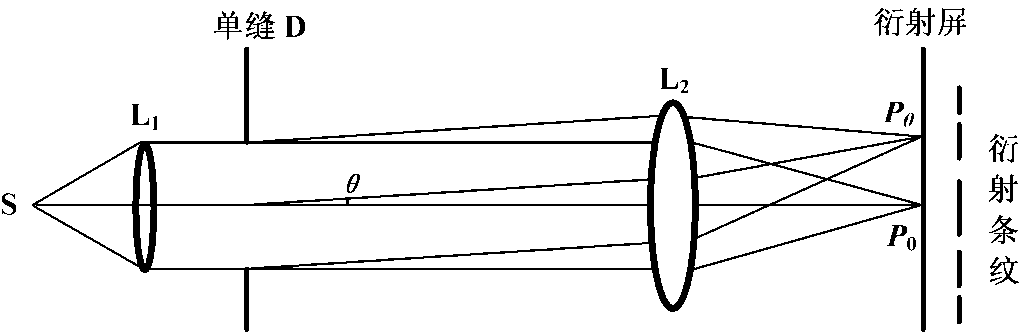
\includegraphics[width=\textwidth]{夫琅禾费光路图.png}
\end{figure}
\end{question}

\begin{question}
    夫琅和费衍射条纹的特点?暗条纹的衍射角与缝宽有什么关系?当缝宽增加一倍或减半,衍射光强和条纹宽度将如何变化?
    \tcblower
    \begin{enumerate}
        \item 当$\theta=0$时,$I=I_0$,这是与光轴平行的光线会聚点的光强,是衍射图像中光强的极
        大值,称为主极大,大部分能量都落在主极大上。
        \item 当$\sin\theta=k\lambda/a(k=\pm1,\pm2\cdots)$时,$I_\theta=0$出现暗条纹。因$\theta$很小,有$\theta\approx \sin\theta$,因此
        可近似认为暗条纹在
        \begin{align*}
            \theta=\frac{k\lambda}{a}
        \end{align*}
        的位置上。可见:\begin{enumerate}
            \item 衍射角$\theta$ 与缝宽$a$ 成反比关系,缝加宽时,衍射角减小,各级条纹向中央收缩;当
            缝宽$a$足够大($a\gg\lambda$)时,衍射现象不明显,从而可以忽略不计,将光看成是沿直
            线传播的。
            \item 中央亮条纹的宽度由k=±1 的两个暗条纹的衍射角所确定,即中央亮条纹的角宽度
            为$\Delta\theta=2\lambda/a$.
            \item 对于任意两条相邻暗条纹,其衍射角的差值为$\Delta\theta=\lambda/a$,即暗条纹是以$P_0$ 为中心,
            等间隔地,左右对称地分布的。
        \end{enumerate}
        \item 两相邻暗条纹之间的是各级亮条纹,它们的宽度是中央亮条纹宽度的二分之一。
        这些亮条纹的光强最大值称为次极大。
    \end{enumerate}
    当缝宽增加一倍时,光强增加,条纹宽度变为原来一半。当缝宽减半时,光强减小,条纹宽度变为原来两倍。
\end{question}



\clearpage
\setLhead{中山大学物理与天文学院基础物理实验记录}
\begin{table}
	\renewcommand\arraystretch{1.7}
	\centering
	\begin{tabularx}{\textwidth}{|X|X|X|X|}
	\hline
	专业:& 物理学类 &年级:& 2023级 \\
	\hline
	姓名: &姚昊廷& 学号:&22322091  \\
	\hline
	室温:&$22^\circ$C&实验地点:&A508  14\\
	\hline
	学生签名:& & 评分: &\\
	\hline
	实验时间:& 2024.11.28& 教师签名:&\\
	\hline
	\end{tabularx}
\end{table}
\section{单缝衍射的相对光强分布\ \textbf{实验记录}}
\subsection{实验内容、步骤、结果}
\noindent 一、	测量单缝衍射的相对光强分布
\begin{question}
    观测单缝衍射条纹分布与狭缝宽度的关系,简单描述当狭缝改变宽度时,观测到的衍射条纹有什么变化 ?简单描述如何判断衍射条纹的主极大。
    \tcblower
    变化:狭缝宽度变大时,衍射条纹变宽,且各级条纹向主极大汇聚。狭缝宽度变小时,衍射条纹变窄,且各级条纹向主极大远离。\\
	判断方法:\begin{enumerate}
		\item 用光屏先看亮条纹,居中最亮的为主极大
		\item 用光功率计在后面对准
		\item 撤去光屏,移动光功率计,使得读数最大,此时即为主极大
	\end{enumerate}
\end{question}
\noindent 1.在X的一个方向每隔(0.1-0.3 mm)上测光强,从主极大一直测到第三条暗纹,记录衍射条纹的光强。\\
激光出光口位置:27.90cm\hspace{4pt}探头位置:87.75cm\hspace{4pt}狭缝位置:40.00cm\hspace{4pt}狭缝宽度:0.015mm
\begin{table}[H]
    \centering
	\caption{单缝衍射的相对光强分布(第一组数据)}
    \begin{tabular}{|l|l|l|l|l|l|}
    \hline
		位置/mm&光功率/$\mu$W&位置/mm&光功率/$\mu$W&位置/mm&光功率/$\mu$W\\ \hline
        0 & 86.8 & 6.6 & 0.479 & 13.2 & 0.141 \\ \hline
        0.3 & 86.9 & 6.9 & 0.62 & 13.5 & 0.209 \\ \hline
        0.6 & 86.2 & 7.2 & 0.9 & 13.8 & 0.324 \\ \hline
        0.9 & 83 & 7.5 & 1.395 & 14.1 & 0.446 \\ \hline
        1.2 & 80.3 & 7.8 & 2.01 & 14.4 & 0.563 \\ \hline
        1.5 & 76.4 & 8.1 & 2.75 & 14.7 & 0.676 \\ \hline
        1.8 & 71.1 & 8.4 & 3.03 & 15 & 0.731 \\ \hline
        2.1 & 64.7 & 8.7 & 3.43 & 15.3 & 0.752 \\ \hline
        2.4 & 58.9 & 9 & 3.66 & 15.6 & 0.755 \\ \hline
        2.7 & 52.1 & 9.3 & 3.72 & 15.9 & 0.538 \\ \hline
        3 & 45.6 & 9.6 & 3.69 & 16.2 & 0.566 \\ \hline
        3.3 & 37 & 9.9 & 3.52 & 16.5 & 0.483 \\ \hline
        3.6 & 30.2 & 10.2 & 3.2 & 16.8 & 0.276 \\ \hline
        3.9 & 25.3 & 10.5 & 2.85 & 17.1 & 0.187 \\ \hline
        4.2 & 19.1 & 10.8 & 2.35 & 17.4 & 0.188 \\ \hline
        4.5 & 15.27 & 11.1 & 1.92 & 17.7 & 0.113 \\ \hline
        4.8 & 11.16 & 11.4 & 1.493 & 18 & 0.066 \\ \hline
        5.1 & 7.8 & 11.7 & 0.913 & 18.3 & 0.033 \\ \hline
        5.4 & 4.55 & 12 & 0.619 & 18.6 & 0.016 \\ \hline
        5.7 & 3.02 & 12.3 & 0.373 & 18.9 & 0.011 \\ \hline
        6 & 1.349 & 12.6 & 0.212 & 19.2 & 0.013 \\ \hline
        6.3 & 0.823 & 12.9 & 0.139 & 19.5 & 0.017 \\ \hline
    \end{tabular}
\end{table}

\noindent 2.改变狭缝宽度,按照上述步骤,再测一组数据。\\
激光出光口位置:18.70cm\hspace{4pt}探头位置:26.25cm\hspace{4pt}狭缝位置:88.2cm\hspace{4pt}狭缝宽度:0.16mm
\begin{table}[H]
    \centering
	\caption{单缝衍射的相对光强分布(第二组数据)}
    \begin{tabular}{|l|l|l|l|l|l|}
    \hline
	位置/mm&光功率/$\mu$W&位置/mm&光功率/$\mu$W&位置/mm&光功率/$\mu$W\\ \hline
        0 & 19.5 & 1.6 & 0.744 & 3.2 & 0.113 \\ \hline
        0.1 & 19.7 & 1.7 & 0.704 & 3.3 & 0.111 \\ \hline
        0.2 & 19.3 & 1.8 & 0.633 & 3.4 & 0.12 \\ \hline
        0.3 & 18.6 & 1.9 & 0.503 & 3.5 & 0.132 \\ \hline
        0.4 & 17.6 & 2 & 0.373 & 3.6 & 0.234 \\ \hline
        0.5 & 16.6 & 2.1 & 0.24 & 3.7 & 0.266 \\ \hline
        0.6 & 13.91 & 2.2 & 0.221 & 3.8 & 0.246 \\ \hline
        0.7 & 10.93 & 2.3 & 0.293 & 3.9 & 0.109 \\ \hline
        0.8 & 8.48 & 2.4 & 0.489 & 4 & 0.093 \\ \hline
        0.9 & 5.91 & 2.5 & 0.681 & 4.1 & 0.08 \\ \hline
        1 & 2.93 & 2.6 & 0.759 & 4.2 & 0.072 \\ \hline
        1.1 & 2.42 & 2.7 & 0.679 & 4.3 & 0.072 \\ \hline
        1.2 & 1.533 & 2.8 & 0.493 & 4.4 & 0.077 \\ \hline
        1.3 & 1.064 & 2.9 & 0.275 & 4.5 & 0.083 \\ \hline
        1.4 & 0.85 & 3 & 0.161 & ~ & ~ \\ \hline
        1.5 & 0.778 & 3.1 & 0.131 & ~ & ~ \\ \hline
    \end{tabular}
\end{table}

\noindent 二、测量点光源光功率与距离的关系 
\begin{table}[H]
	\centering
	\caption{光源光功率与距离的关系}
	\begin{tabular}{cc}
		\toprule
		光探头与光源的距离X/cm&光功率/$\mu$W\\
		\midrule
		25&46.3\\
		30&32.8\\
		35&24.3\\
		40&18.5\\
		45&14.62\\
		50&12.03\\
		55&10.19\\
		60&8.44\\
		65&7.35\\
		70&6.34\\
		75&5.27\\
		80&4.86\\
		\toprule
	\end{tabular}
\end{table}
\subsection{实验过程中遇到的问题记录}
\begin{enumerate}
	\item 光功率计不灵敏,读数不完全准确,会受上一个位置光强影响
	\item 较难测得各出口位置
\end{enumerate}


\clearpage
\setLhead{中山大学物理与天文学院基础物理实验分析与讨论}
\begin{table}
	\renewcommand\arraystretch{1.7}
	\begin{tabularx}{\textwidth}{|X|X|X|X|}
	\hline
	专业:& 物理学 &年级:& 2023级\\
	\hline
	姓名: &姚昊廷& 学号:&22322091 \\
	\hline
    日期:&2024.11.28 & 评分: &\\
	\hline
	\end{tabularx}
\end{table}

\section{单缝衍射的相对光强分布\ \textbf{分析与讨论}}
\begin{question}
	讨论你的实验是否满足夫琅和费衍射条件。
	\tcblower
第一组有:$\dfrac{a_1^2}{8Z\lambda}=0.00816\gg 1$\\
第二组有:$\dfrac{a_2^2}{8Z\lambda}=0.0287\gg 1$\\
故均满足夫琅禾费衍射条件
\end{question}

\begin{question}
	根据测得的数据,利用计算机软件做出激光单缝衍射相对光强分布曲线。
	\tcblower
	\begin{figure}[H]
		\includegraphics[width=0.5\textwidth]{1.png}
		\includegraphics[width=0.5\textwidth]{2.png}
	\end{figure}
\end{question}

\begin{question}
	计算实测得到的光强分布曲线中各次极大光强与主极大光强的比值,与理论值比较。讨论有差异的原因。
	\tcblower
	\begin{table}[H]
		\centering
		\begin{tabular}{|l|l|l|l|l|}
		\hline
		&理论值&实验1&与理论值绝对误差&与理论值相对误差\\ \hline
		主极大&1&1&&\\
		\hline
		第一次极大&0.0469&0.0385&-0.0084&-17.9\%\\
		\hline
		第二次极大&0.0166&0.0135&-0.0031&-18.7\%\\
		\hline
		\end{tabular}
		\begin{tabular}{|l|l|l|}
			\hline
			实验2&与理论值绝对误差&与理论值相对误差\\ \hline
			1&&\\
			\hline
			0.0270&-0.0199&-42.4\%\\
			\hline
			0.0098&-0.0068&-41.0\%\\
			\hline
		\end{tabular}
	\end{table}
	原因:\begin{enumerate}
		\item 系统误差:\begin{enumerate}
			\item 实验未严格满足夫琅禾费衍射条件
			\item 光功率计不灵敏,读数不完全准确,会受上一个位置光强影响
			\item 步长太大错过最大值
		\end{enumerate}
		\item 随机误差:\begin{enumerate}
			\item 光功率计读数有变化
			\item 光探头位置读数不严格
		\end{enumerate}
	\end{enumerate}
\end{question}

\begin{question}
	根据得到的光强分布曲线,计算各衍射暗条纹对应的衍射角,计算出狭缝宽度。
	\tcblower
	\begin{table}[H]
		\centering
		\caption{第一组}
		\begin{tabular}{|l|l|l|l|}
		\hline
		&位置x/mm&衍射角$\theta$&狭缝宽$a=\frac{k\lambda}{\sin\theta}$\\
		\hline
		第一条暗纹&3.8&$0.35^\circ$&0.103\\
		\hline
		第二条暗纹&6&$0.55^\circ$&0.131\\
		\hline
		第三条暗纹&7.8&$0.72^\circ$&0.151\\
		\hline
		\end{tabular}
	\end{table}
	\begin{table}[H]
		\centering
		\caption{第二组}
		\begin{tabular}{|l|l|l|l|}
		\hline
		&位置x/mm&衍射角$\theta$&狭缝宽$a=\frac{k\lambda}{\sin\theta}$\\
		\hline
		第一条暗纹&4&$0.37^\circ$&0.098\\
		\hline
		第二条暗纹&5.3&$0.49^\circ$&0.148\\
		\hline
		第三条暗纹&6.5&$0.60^\circ$&0.181\\
		\hline
		\end{tabular}
	\end{table}
	即第一组宽度$\overline{a}_1=0.128mm$与实际值相对误差$\dfrac{\overline{a}_1-a_1}{a_1}=-20\%$\\
	即第二组宽度$\overline{a}_2=0.142mm$与实际值相对误差$\dfrac{\overline{a}_2-a_2}{a_2}=-29\%$\\
	误差来源可能有:\begin{enumerate}
		\item 光功率计不灵敏,在第一暗纹处极小值在下降
		\item 在第一暗纹受主极大影响导致第一暗纹偏大
	\end{enumerate}
\end{question}

\begin{question}
	利用计算机软件作光功率与距离平方倒数的关系曲线,验证点光源是否满足光功率与距离平方的反比关系。
	\tcblower
\begin{figure}[H]
	\includegraphics[width=\textwidth]{3.png}
\end{figure}
$R^2=0.99976$故点光源满足光功率与距离平方反比关系。
\end{question}
\subsection{附加实验结果}
\noindent 1.测试头发宽度\\
步骤:\begin{enumerate}
	\item 将头发拉直到激光器前,使光屏上出现衍射条纹
	\item 测量主极大到第三条暗纹之间的距离
	\item 记录激光器出光口与光屏距离
	\item 使用公式$\sin\theta=\frac{k\lambda}{a}$计算头发宽度
\end{enumerate}
代入所测得数据$x=12.5mm,z=69.05cm$后得到头发宽度$a=90.42\mu m$
\subsection{实验后思考题}
\begin{question}
	使用光功率计应注意哪些问题?光功率计进光狭缝的宽度对实验结果有何影响?
	\tcblower
	注意:\begin{enumerate}
		\item 光功率计应确保光屏紧贴狭缝后,不漏光。
		\item 有效数字小于三位后应及时换档。
	\end{enumerate}
	影响:\begin{enumerate}
		\item 若狭缝过宽,对光条纹强度的极大值和极小值测量不明显
		\item 若过窄,则环境噪声影响加大,读数困难且波动大
	\end{enumerate}
\end{question}

\begin{question}
	能否用激光光源研究光源光功率与距离平方的反比关系?
	\tcblower
	不能,光功率与距离平方的反比关系仅适用于球面光,激光方向性好,发散角度小,几乎沿平行方向发射,短距离内无法观测到光功率减弱,因此不能实验激光光源。
\end{question}
\clearpage
% ---------------------------------------------------------------------
%   参考文献
%   注:使用参考文献时应按照xelatex->bibtex->xelatex->xelatex顺序进行编译
%\phantomsection
%\addcontentsline{toc}{section}{参考文献}
%\bibliographystyle{unsrt}
%\bibliography{myref}
%\begin{thebibliography}{9}
%	\bibitem{ref1} 沈雨欣,翁存程,蒋丽钦.双棱镜干涉法准确测量钠光波长[J].大学物理实验,2023,36(03):40-43.DOI:10.14139/j.cnki.cn22-1228.2023.03.008.
%	\bibitem{ref2} 牟泉润,孙丽媛,杜月棋,等.基于干涉原理的光波长测量装置设计[J].大学物理实验,2021,34(06):80-83+89.DOI:10.14139/j.cnki.cn22-1228.2021.06.018.
%	\bibitem{ref3} 王仁洲,杨涛.一种用激光干涉测量光波波长的新方法[J].大学物理实验,2014,27(06):41-43.DOI:10.14139/j.cnki.cn22-1228.2014.06.014.
%\end{thebibliography}


%\clearpage
\appendix
\appendixpage
\addappheadtotoc
%\subsection*{相图代码}
%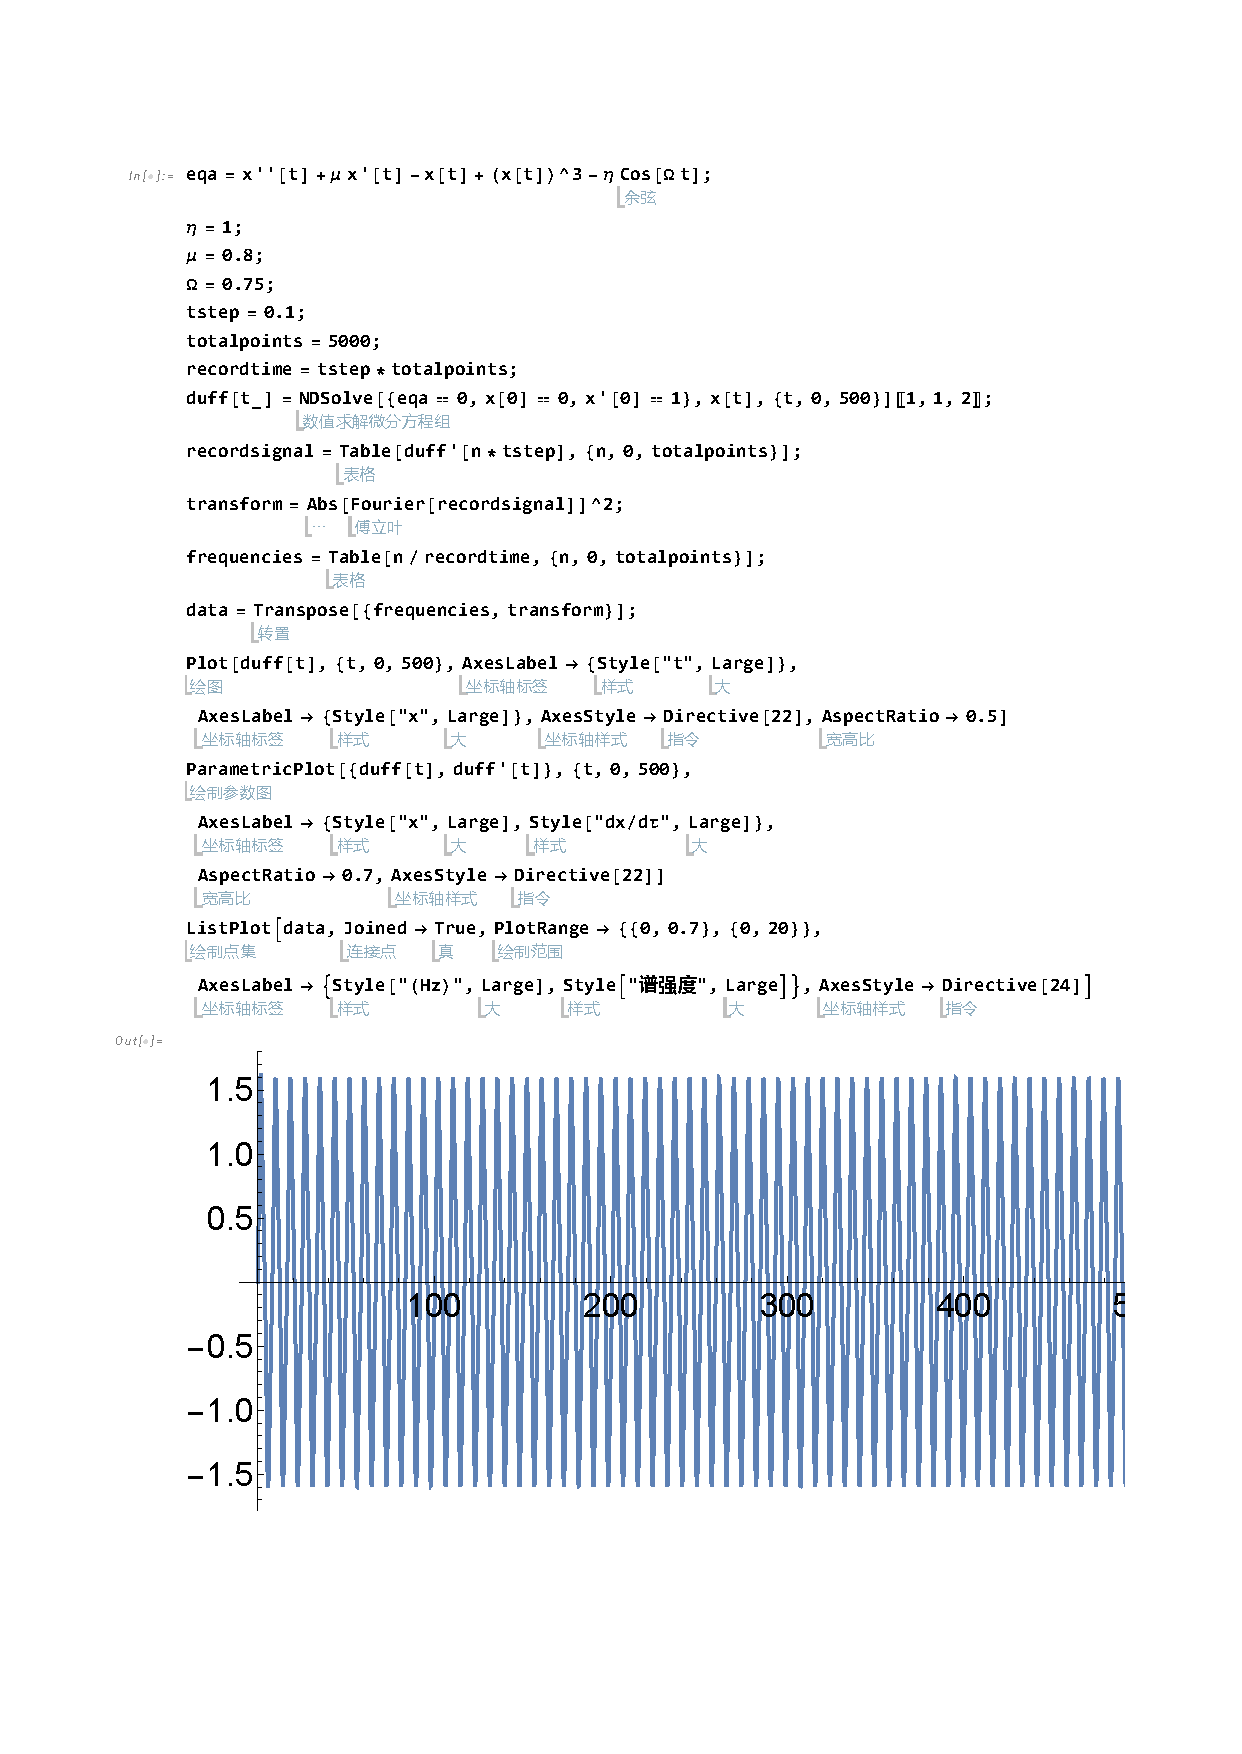
\includepdf[pages=-]{chaos.pdf}
\subsection*{原件}
%
\includepdf[pages=-]{实验3原件.pdf}
%\begin{figure}[H]
%	\centering
%	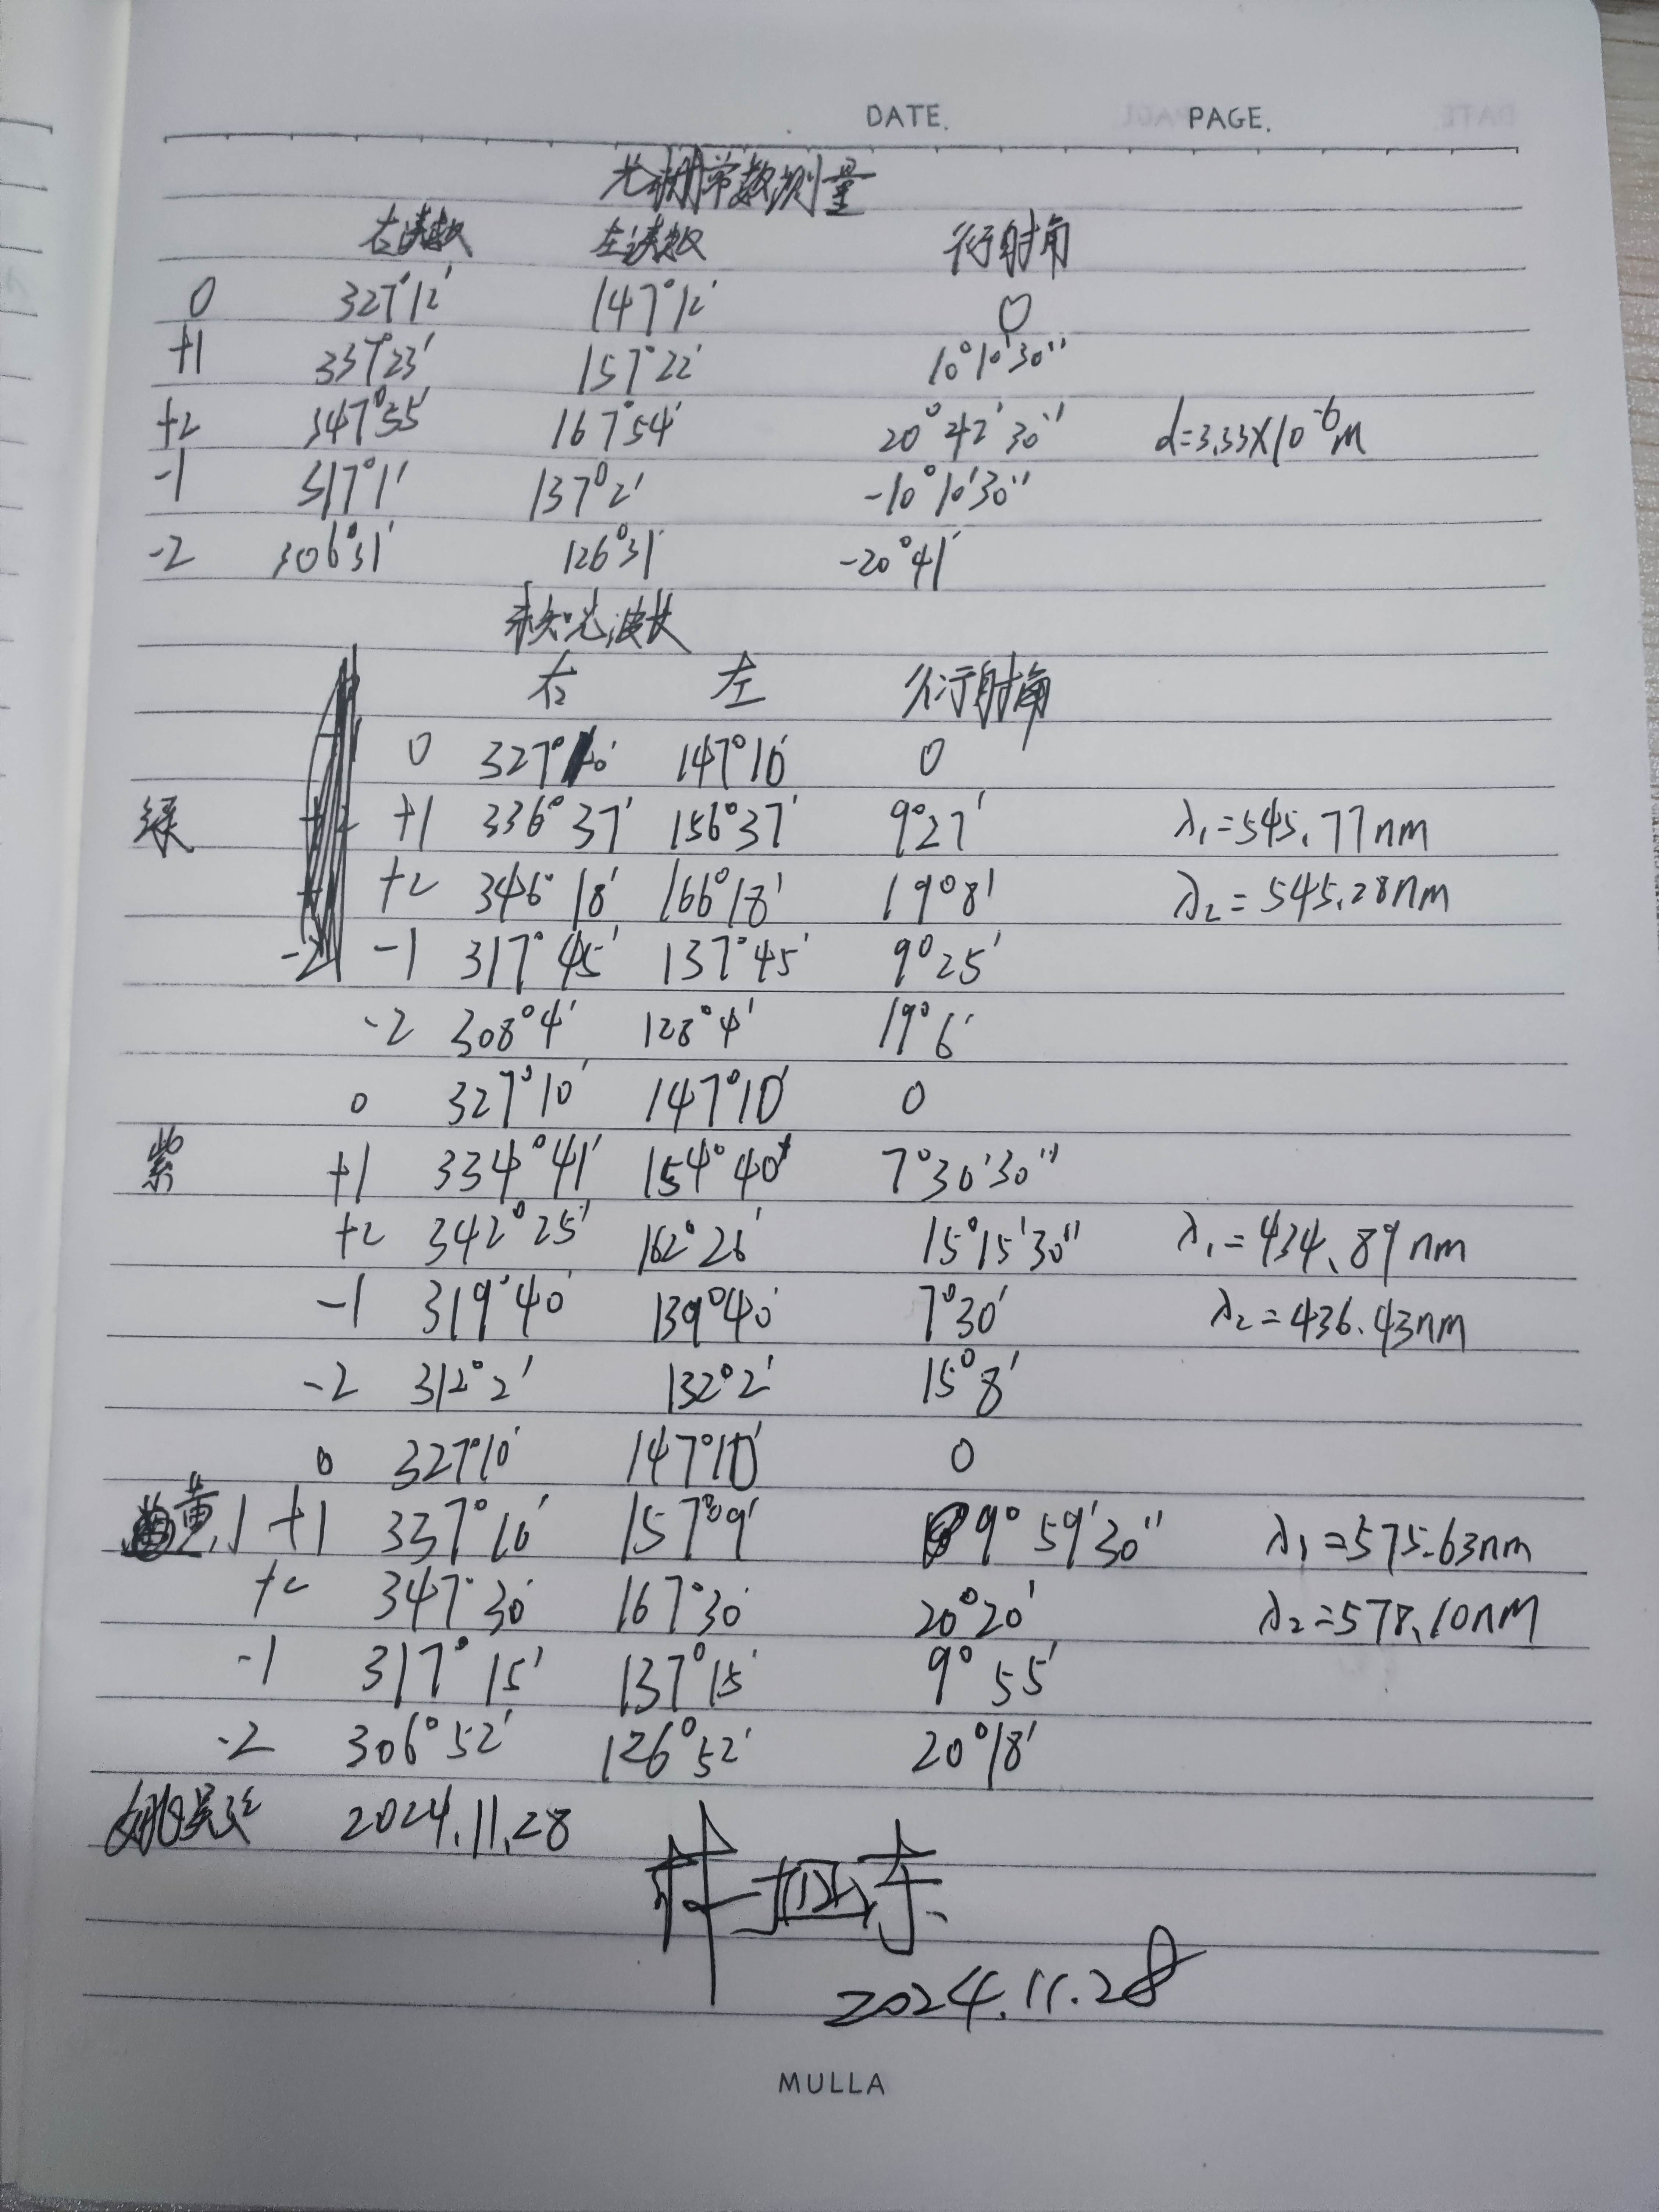
\includegraphics[width=\textwidth]{光栅数据.jpg}
%\end{figure}

\begin{figure}[H]
	\centering
	\includegraphics[width=0.4\textwidth]{单缝原件1.jpg}
	\includegraphics[width=0.4\textwidth]{单缝原件2.jpg}
	\includegraphics[width=0.4\textwidth]{单缝原件3.jpg}
	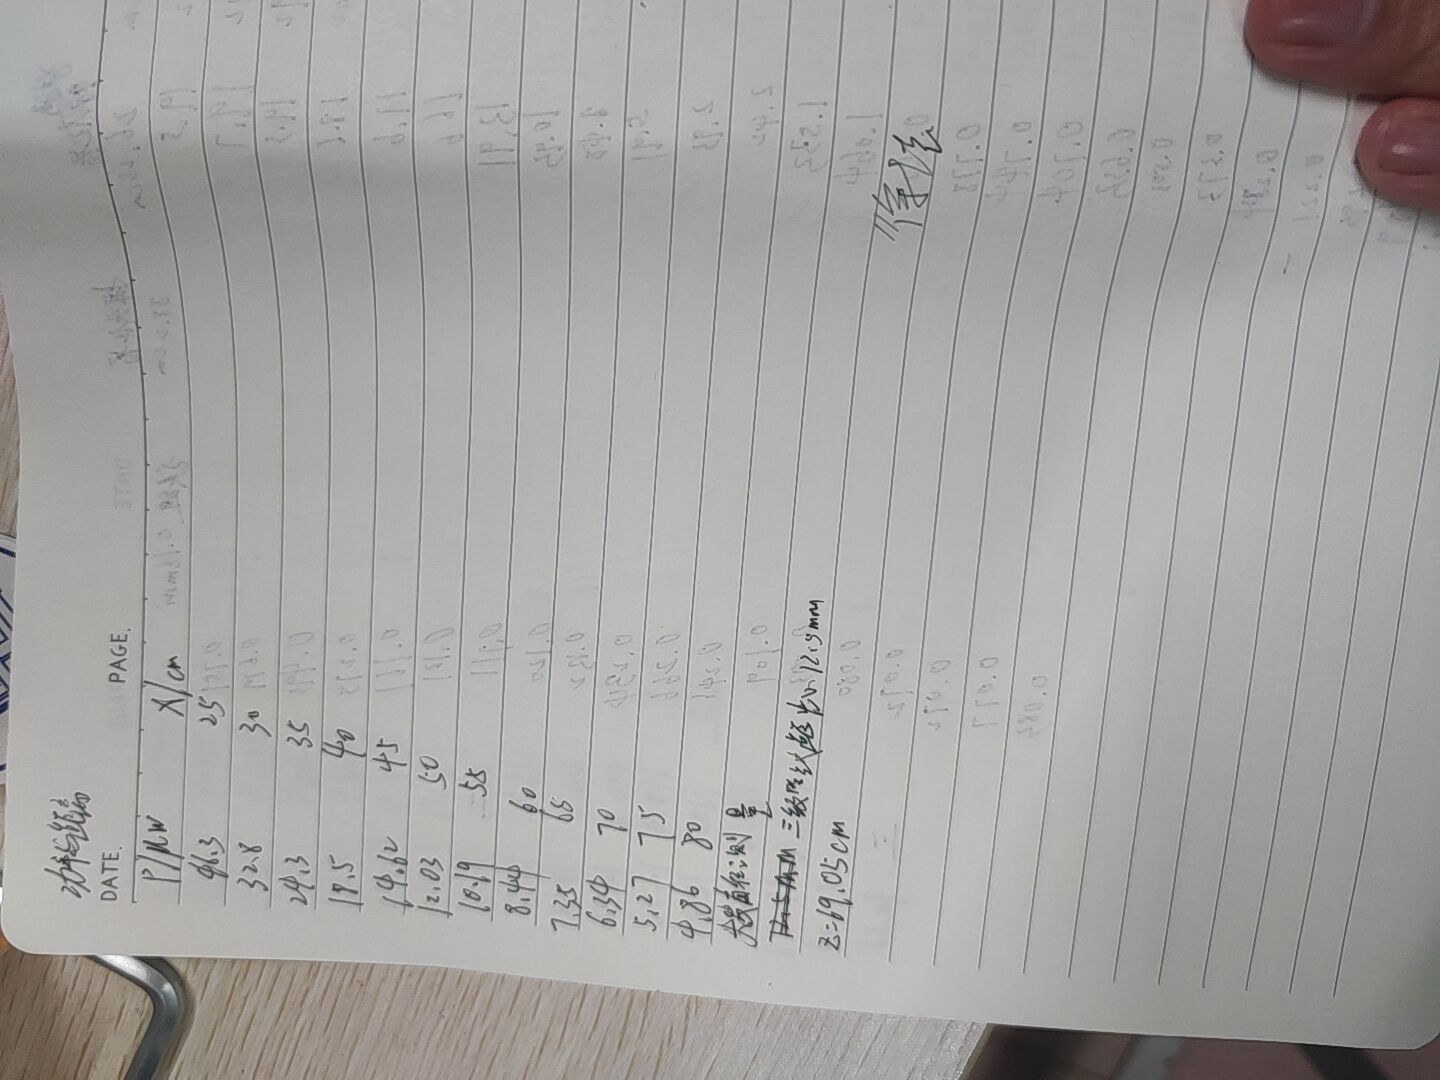
\includegraphics[width=0.4\textwidth]{单缝原件4.jpg}
\end{figure}
\subsection*{桌面}
\begin{figure}[H]
	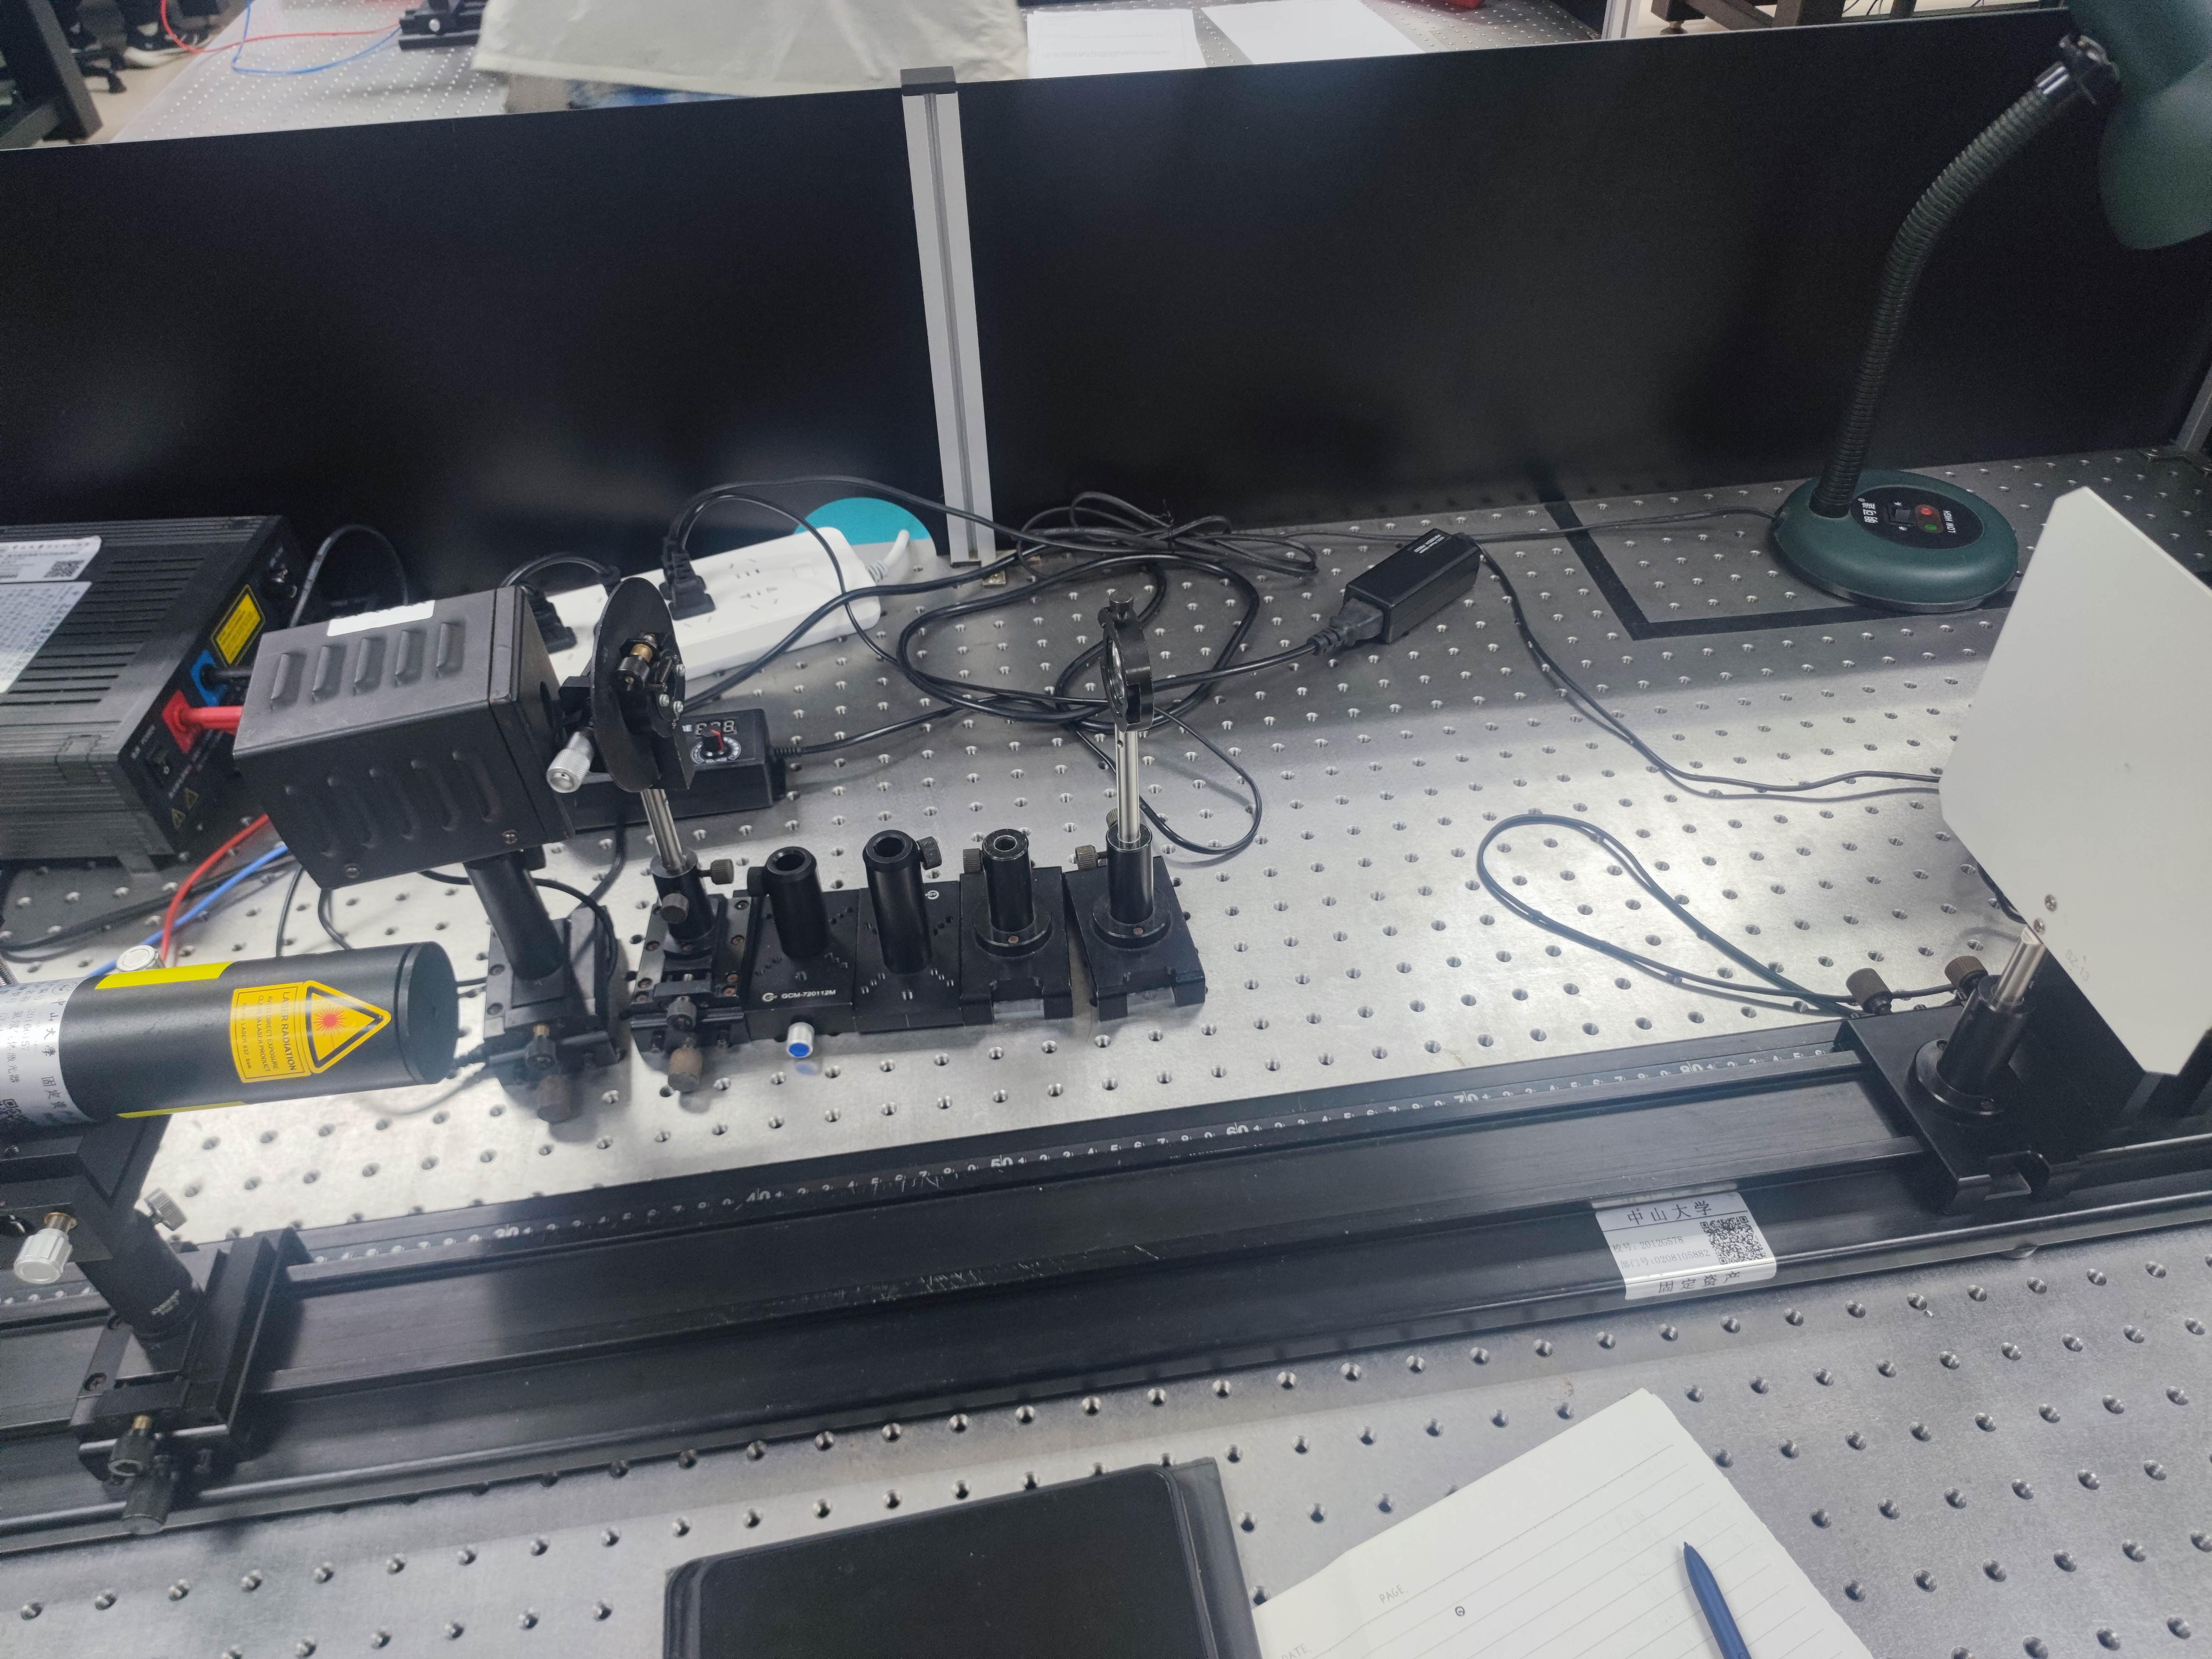
\includegraphics[width=0.95\textwidth]{单缝桌面.jpg}
\end{figure}
\end{document}
%